
\section*{Ejercicio 2}
\subsection{Análisis teórico}
El circuito a analiza consiste, a grandes rasgos, en un amplificador no inversor.
Para su estudio teórico se tomarán dos modelos, donde, en primer lugar, se considerará al amplificador operacional en su versión ideal, para luego introducir no idealidades en su impedancia de entrada, salida y en la ganancia del mismo.
Los valores de las resistencias a utilizar fueron reemplazados por su valor comercial más cercano, resultando en que el circuito a analizar sea el de la figura \ref{fig:initial_circuit}
\begin{figure}[H]
    \begin{minipage}{\textwidth}
        \centering
        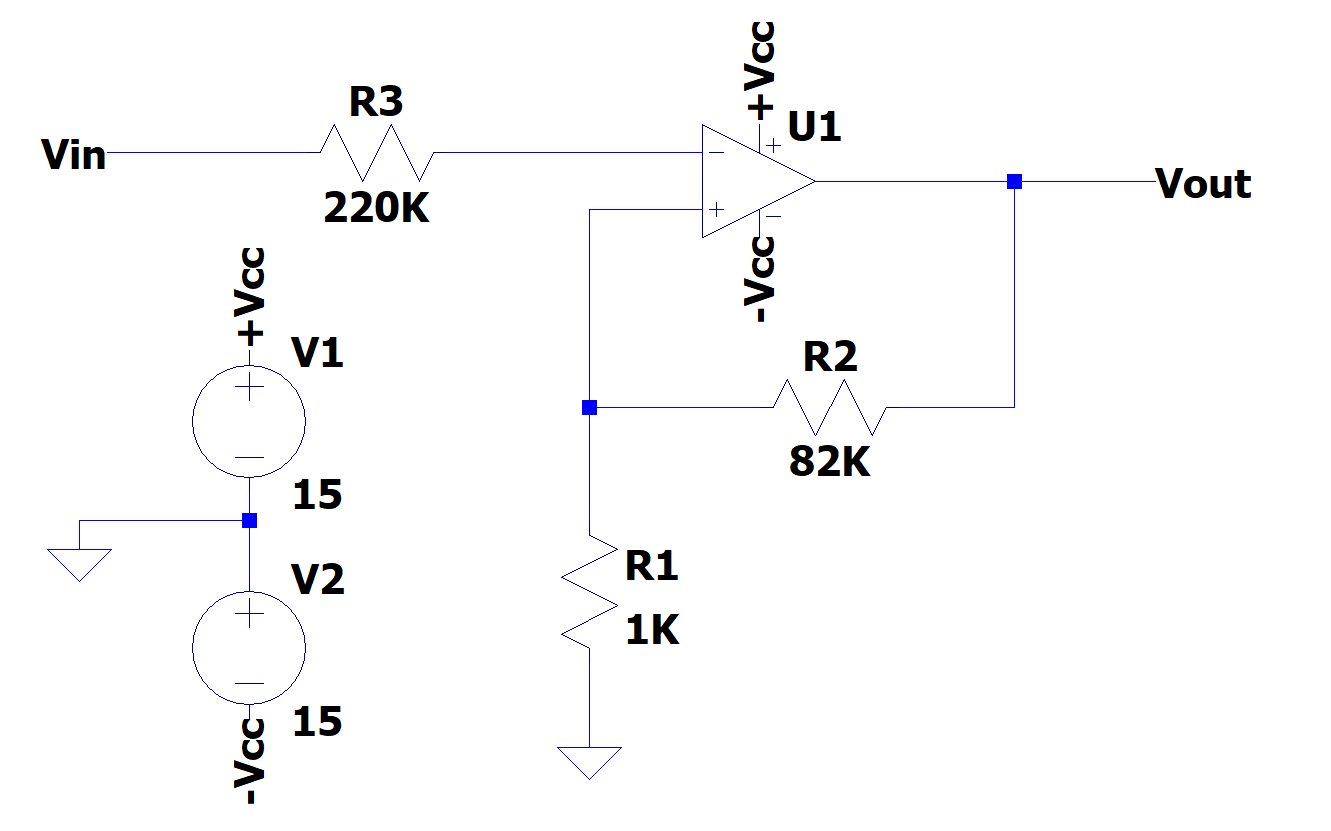
\includegraphics[width=\textwidth]{../EJ2/recursos_para_el_informe/circuito_a_analizar_ideal}
        \caption{Circuito a analizar.}
        \label{fig:initial_circuit}
    \end{minipage}\hfill
\end{figure}


\subsubsection{Modelo ideal}
La primer aproximación al comportamiento del circuito se realizará considerando al amplificador operacional como un componente ideal, es decir, $Av = \inf$, $Z_{in_{opamp}} = \inf$, $Z_{out_{opamp}} = 0$.
De esta manera, sin importar el modelo de operacional utilizado, se tiene que:
\begin{equation}
    \label{eq:ideal_gain}
    \frac{v_{out}}{v_{in}} = 1 + \frac{R_2}{R_1} = 1 + \frac{82 K\Omega}{1 K\Omega} = 83 \implies 38,38 dB
\end{equation}

Se desprende también, de las condiciones de idealidad impuestas, que la impedancia de entrada del circuito será infinita.


\subsubsection{Modelo con impedancia de entrada, salida, y ganancia finita}
Para la resolución del circuito con las consideraciones ya mencionadas, es necesario ahora especificar qué datos serán utilizados para los cálculos.
Los mismos fueron obtenidos de las correspondientes datasheets 
\footnote{Datasheet para operacional LM833: https://www.ti.com/lit/ds/symlink/lm833.pdf \\Datasheet para operacional NE5534: https://www.onsemi.com/pub/Collateral/NE5534-D.PDF}, 
y se presentan en el cuadro \ref{tab:parameters_for_equations}.
\begin{table}[H]
    \label{tab:parameters_for_equations}
    \centering
    \begin{tabular}{|l|llll|}
        \hline
        \textbf{\begin{tabular}[c]{@{}l@{}}Modelo de operacional\end{tabular}} & \textbf{\begin{tabular}[c]{@{}l@{}}$f_0$ (Hz)\end{tabular}} & \textbf{\begin{tabular}[c]{@{}l@{}}$A_0$ \end{tabular}} & \textbf{$Z_{in_{opamp}}(K\Omega)$} & \textbf{$Z_{out_{opamp}}(\Omega)$} \\ \hline
        \textbf{LM833}                                                         & $16 \cdot 10^3$                                             & $1000$                                                  & $175$                              & $37$                               \\
        \textbf{NE5534}                                                        & $100$                                                       & $10 \cdot 10^5$                                         & $100$                              & $0,3$                              \\ \hline
        \end{tabular}
    \caption{Parámetros para cálculo de circuito no ideal.}
\end{table}

Se modelizará al operacional mediante el circuito \ref{fig:non_ideal_circuit}
\begin{figure}[H]
    \begin{minipage}{\textwidth}
        \centering
        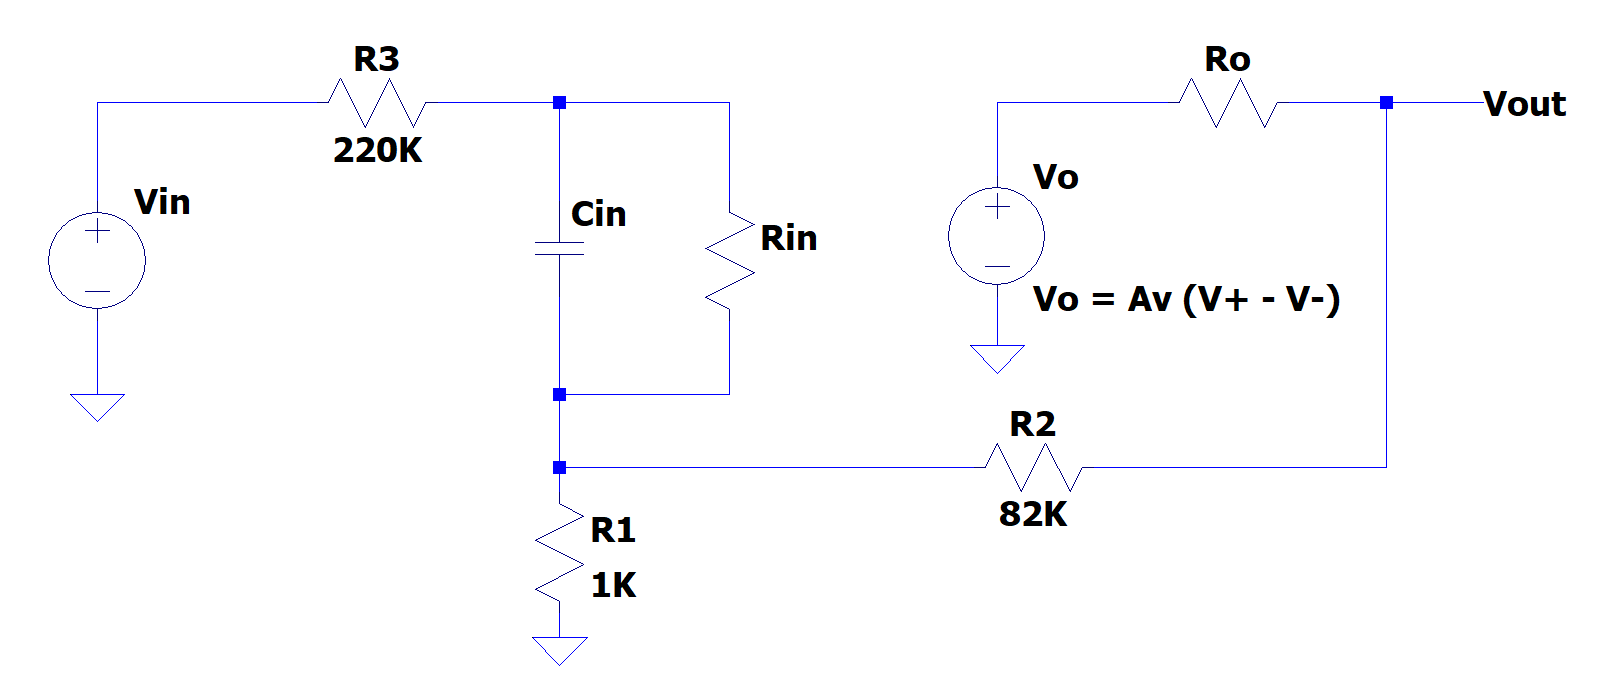
\includegraphics[width=\textwidth]{../EJ2/recursos_para_el_informe/circuito_a_analizar_no_ideal}
        \caption{Circuito a analizar.}
        \label{fig:non_ideal_circuit}
    \end{minipage}\hfill
\end{figure}

Se entiende al circuito como dos mallas cuyas ecuaciones son las descriptas en \ref{eq:system_meshes}, que se extraen del circuito \ref{fig:meshes_circuit}
\begin{figure}[H]
    \begin{minipage}{\textwidth}
        \centering
        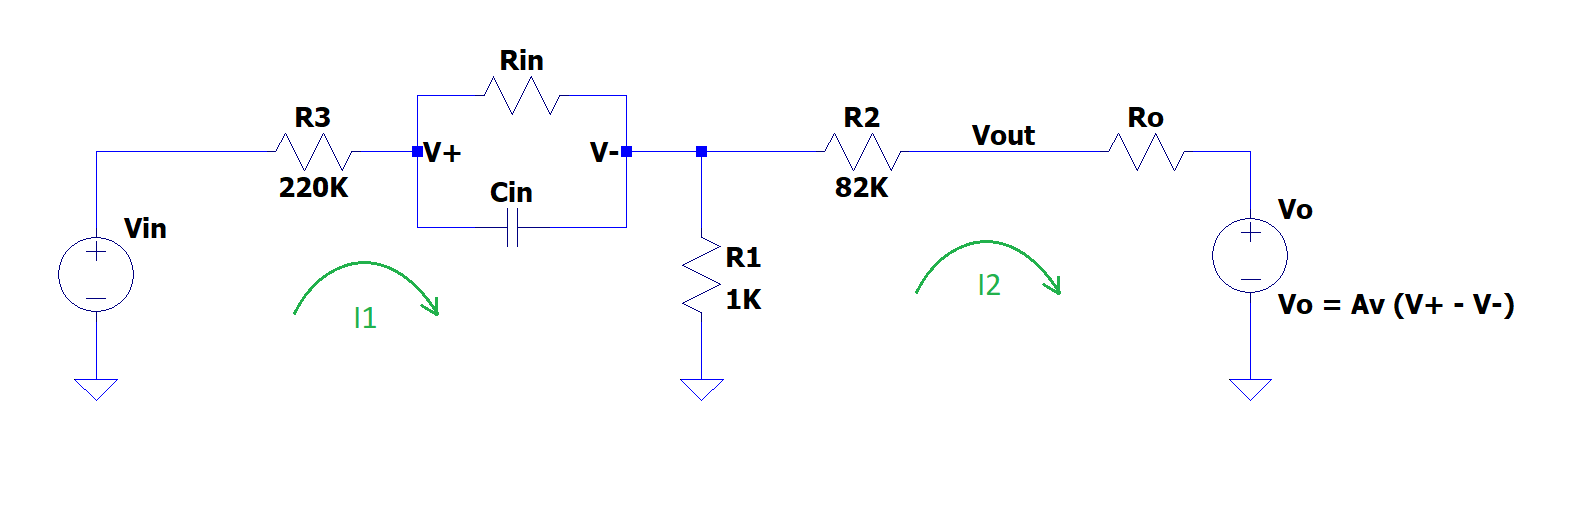
\includegraphics[width=\textwidth]{../EJ2/recursos_para_el_informe/circuito_mallas}
        \caption{Circuito a analizar.}
        \label{fig:meshes_circuit}
    \end{minipage}\hfill
\end{figure}

\begin{align}
    &v_{in} - i_1 \cdot R_3 - i_1 \cdot Z_{in} - \left(i_1 - i_2\right) \cdot R_1 = 0 \\
    &-\left(i_2 - i_1\right) \cdot R_1 - i_2 \cdot R_2 - I_2 \cdot R_0 - v_o = 0 \\
    &v_o = \left(v^+ - v^-\right) \cdot A_v \\
    &v^+ = v_{in} - i_1 \cdot R_3 \\
    &v^- = v_{in} - i_1 \cdot R_3 - i_1 \cdot Z_{in} \\
    &Z_{in} = \frac{R_{in}}{R_{in} \cdot C_{in} \cdot s + 1} \label{eq:zin} \\
    &A_v = \frac{A_0}{1+\frac{s}{\omega_p}}
    \label{eq:system_meshes}
\end{align}

Resolviendo para $i_2$ se obtiene que:
\begin{equation}
    i_2 = v_{in} \cdot \frac{R_1 - A_v \cdot Z_{in}}{R1 \cdot \left(A_v \cdot Z_{in} - R_1\right) + \left(R_3 + Z_{in} + R_1\right) \cdot \left(R_1 + R_2 + R_o\right)}
    \label{eq:i2}
\end{equation}

Y luego se expresan $v_{out}$ e $i_1$ en función de $i_2$, a fin de evitar largas expresiones, como:
\begin{align}
    &i_1 = \frac{v_{in} + i_2 \cdot R_1}{R_3 + Z_{in} + R_1} \\
    &v_{out} = v_{in} \cdot \frac{R_1}{R_3 + Z_{in} + R_1} + i_2 \cdot \frac{R_1^2}{R_3 + Z_{in} + R_1} + i_2 \cdot R_1 - i_2 \cdot R_2
    \label{eq:i1_and_vout}
\end{align}

